% Build with pdflatex training_plan_en.tex (twice).
\documentclass[11pt,a4paper]{article}
\usepackage[T1]{fontenc}
\usepackage{tgpagella}
\usepackage[scale=.94]{tgheros}
\usepackage[margin=19mm,top=19mm,bottom=20mm,footskip=10mm]{geometry}
\usepackage{amsmath,microtype,booktabs,array,tabularx,tikz,fancyhdr}
\usetikzlibrary{arrows.meta,calc}
\usepackage[hidelinks]{hyperref}
\hypersetup{pdftitle={Traffic Signal Control: Training and Evaluation Plan},pdfauthor={CBWCE experiment}}
\definecolor{ink}{HTML}{182E35}
\definecolor{sea}{HTML}{14675F}
\definecolor{mist}{HTML}{EAF4EF}
\definecolor{sand}{HTML}{FAF0DD}
\definecolor{ochre}{HTML}{87541E}
\definecolor{linecol}{HTML}{66847F}
\definecolor{pale}{HTML}{F2F5F6}
\color{ink}
\pagestyle{fancy}\fancyhf{}\renewcommand{\headrulewidth}{0pt}
\fancyfoot[L]{\small\sffamily Traffic signal control\enspace/\enspace Experimental protocol}
\fancyfoot[R]{\small\sffamily\thepage\,/\,3}
\setlength{\parindent}{0pt}\setlength{\parskip}{5pt}
\newcommand{\pagehead}[2]{{\sffamily\bfseries\color{sea}\small #1\par}\vspace{1mm}{\fontsize{26}{30}\selectfont #2\par}\vspace{2mm}}
\newcommand{\subhead}[1]{\par\vspace{3mm}{\sffamily\bfseries\large\color{sea}#1\par}\vspace{.5mm}}
\newcommand{\thd}[1]{{\sffamily\bfseries #1}}
\newcolumntype{L}[1]{>{\raggedright\arraybackslash}p{#1}}
\newcolumntype{Y}{>{\raggedright\arraybackslash}X}
\newcommand{\tabsetup}{\small\renewcommand{\arraystretch}{1.22}\setlength{\tabcolsep}{5pt}}
% Page 1 uses the full width of A3; subsequent pages use the A4 document layout.
\definecolor{parentblue}{HTML}{24568A}
\definecolor{ice}{HTML}{E7F0FA}
\definecolor{leaf}{HTML}{DDEFE6}
\tikzset{
  cell/.style={align=center,rounded corners=2pt,inner sep=3pt,
    minimum width=4.05cm,minimum height=.88cm,font=\sffamily\normalsize},
  algorithm/.style={cell,fill=ink,text=white,font=\sffamily\bfseries\large},
  parent/.style={cell,fill=ice,draw=parentblue,text=parentblue},
  demand/.style={cell,fill=sand,draw=ochre,text=ochre},
  branch/.style={cell,fill=leaf,draw=sea,text=ink},
  basewire/.style={draw=parentblue,line width=1pt},
  wcewire/.style={draw=ochre,line width=1.1pt,densely dashed},
  tip/.style={-{Stealth[length=2.3mm,width=2mm]}},
  rowlabel/.style={anchor=west,align=left,text width=4.4cm,font=\sffamily\normalsize}
}
% Each lane owns both checkpoints; unique node prefixes prevent cross-map links.
\newcommand{\taskid}[1]{{\bfseries\ifnum\numexpr#1\relax<10 0\fi\number\numexpr#1\relax}}
\newcommand{\lane}[4]{%
  \begin{scope}[xshift=#1cm]
    \node[algorithm] (#2alg) at (0,-1.65) {#3};
    \node[parent] (#2parent) at (0,-3.40) {\taskid{#4}\enspace Baseline};
    \node[demand] (#2wce) at (0,-5.38) {\taskid{#4+6}\enspace Offline WCE};
    \draw[draw=ink,tip] (#2alg)--(#2parent);
    \draw[basewire,tip] (#2parent)--(#2wce);
    \foreach \id/\y/\offset/\method in {base/-7.56/12/Baseline continuation,
      random/-9.02/18/Random group,dr/-10.48/24/Domain randomization,
      fixed/-11.94/30/Fixed WCE,online/-13.40/36/Online WCE}
      \node[branch] (#2\id) at (0,\y) {\taskid{#4+\offset}\enspace \method};
    \coordinate (#2left) at (-2.49,-3.40);
    \draw[basewire] (#2parent.west)--(#2left)--(#2left |- #2online.west);
    \foreach \id in {base,random,dr,fixed,online}
      \draw[basewire,tip] (#2left |- #2\id.west)--(#2\id.west);
    \coordinate (#2right) at (2.49,-5.38);
    \draw[wcewire] (#2wce.east)--(#2right)--(#2right |- #2online.east);
    \foreach \id in {fixed,online}
      \draw[wcewire,tip] (#2right |- #2\id.east)--(#2\id.east);
  \end{scope}}
\newcommand{\maphead}[4]{%
  \node[cell,minimum width=14.8cm,fill=pale,draw=linecol] (#1map) at (#2,0)
    {{\bfseries\large #3}\enspace /\enspace #4 junctions};
  \coordinate (#1fork) at (#2,-.78);
  \draw[draw=ink] (#1map)--(#1fork);
  \foreach \id in {A,B,C}
    \draw[draw=ink,tip] (#1fork)-|(#1\id alg.north);}
\begin{document}
\newgeometry{layoutwidth=420mm,layoutheight=297mm,left=16mm,right=16mm,top=14mm,bottom=17mm,footskip=9mm}
\pdfpagewidth=420mm\pdfpageheight=297mm\setlength{\headwidth}{\textwidth}
\pagehead{01\quad Training workflow\hfill Training seed 101}{42 training tasks across two maps and three algorithms}
\begin{center}
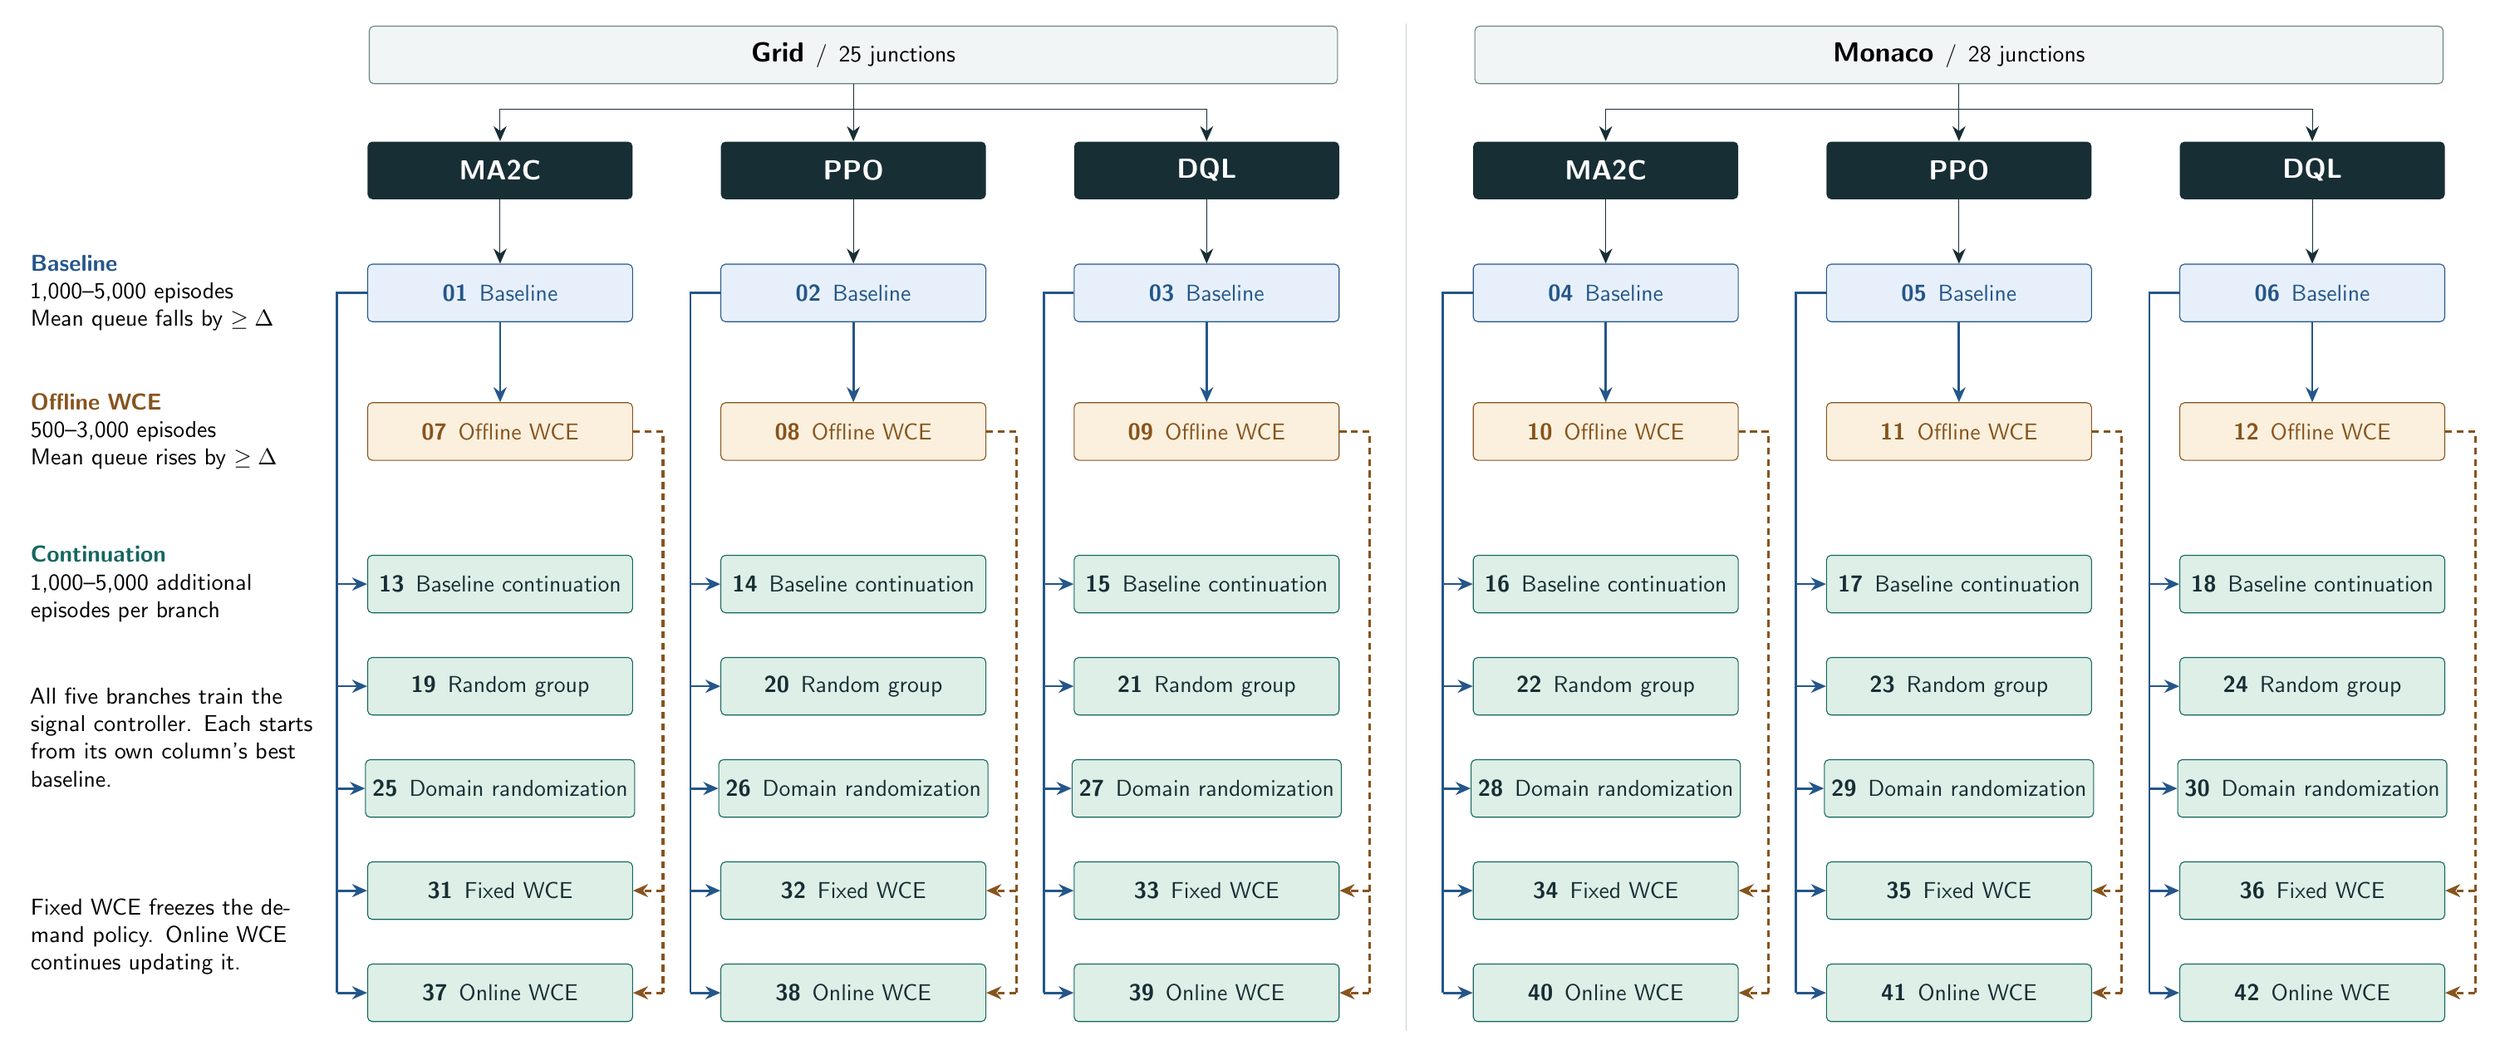
\begin{tikzpicture}[y=1.07cm]
  \lane{7.3}{gA}{MA2C}{1}      \lane{12.7}{gB}{PPO}{2}      \lane{18.1}{gC}{DQL}{3}
  \lane{24.2}{mA}{MA2C}{4}     \lane{29.6}{mB}{PPO}{5}      \lane{35.0}{mC}{DQL}{6}
  \maphead{g}{12.7}{Grid}{25}\maphead{m}{29.6}{Monaco}{28}
  \draw[linecol!35] (21.15,.45)--(21.15,-13.95);
  \node[rowlabel] at (0,-3.40) {\textcolor{parentblue}{\bfseries Baseline}\\1,000--5,000 episodes\\Mean queue falls by $\geq\Delta$};
  \node[rowlabel] at (0,-5.38) {\textcolor{ochre}{\bfseries Offline WCE}\\500--3,000 episodes\\Mean queue rises by $\geq\Delta$};
  \node[rowlabel] at (0,-7.56) {\textcolor{sea}{\bfseries Continuation}\\1,000--5,000 additional episodes per branch};
  \node[rowlabel] at (0,-9.75) {All five branches train the signal controller. Each starts from its own column's best baseline.};
  \node[rowlabel] at (0,-12.6) {Fixed WCE freezes the demand policy. Online WCE continues updating it.};
\end{tikzpicture}
\par\vspace{3mm}{\sffamily
\tikz[baseline=-.5ex]\draw[basewire,tip](0,0)--(1.2,0);\quad Load best baseline controller
\hspace{15mm}
\tikz[baseline=-.5ex]\draw[wcewire,tip](0,0)--(1.2,0);\quad Also load best offline WCE}
\end{center}
\smallskip
\noindent\colorbox{pale}{\begin{minipage}{\dimexpr\linewidth-2\fboxsep}
\centering\sffamily\vspace{3pt}
\textbf{Meaningful improvement}\qquad
$\Delta=\max(\mathrm{anchor}\times 0.01,\;0.1)$ vehicles\qquad
The anchor starts at the episode-0 validation mean queue and resets at each meaningful improvement.\par\smallskip
Validate every 100 episodes. Once the stage minimum is reached, ten consecutive checks without meaningful improvement end training.
Save every new validation best, including smaller improvements.
\vspace{3pt}\end{minipage}}\par
\smallskip
\noindent\colorbox{mist}{\begin{minipage}{\dimexpr\linewidth-2\fboxsep}
\centering\sffamily\vspace{4pt}
\textbf{Controller validation: 11 fixed demand groups per map}\qquad
11 consecutive groups $\times$ 600 seconds = one 6,600-second rollout.\par\smallskip
Each group is a pregenerated, frozen domain-randomization mixture of the 11 original profiles, with weights drawn once from Dirichlet$(1,\ldots,1)$.\par
Reuse the same weights, group order, traffic and simulator/policy seeds across checkpoints, algorithms and continuation methods within each map; use one fixed realization (index 0).\par
Start from an empty network; carry vehicles and controller state across group boundaries. Select the lowest mean queue over the complete 6,600 seconds.\par\smallskip
\textbf{Offline WCE validation:} every 100 episodes, the candidate generates demand against its frozen baseline for one fixed realization (index 0); select the highest mean queue.
\vspace{4pt}\end{minipage}}\par
\restoregeometry
\pdfpagewidth=210mm\pdfpageheight=297mm\setlength{\headwidth}{\textwidth}
\pagehead{02\quad Training settings}{What trains in each step?}
\noindent\colorbox{mist}{\parbox{\dimexpr\linewidth-2\fboxsep}{\centering\sffamily
\strut\textbf{One episode}\enspace =\enspace 11 demand blocks $\times$ 600 simulated seconds = 6,600 seconds\\
\strut Signals act every 5 seconds: 120 joint decisions per block, 1,320 per episode.}}
\subhead{1. Train the baseline controller\hfill\normalfont\small 1,000--5,000 episodes}
Use each of the map's 11 original demand groups once per episode in a fixed order. A group describes where vehicles enter and where they are headed. Queues and vehicles carry over when the group changes.

{\tabsetup\begin{tabularx}{\linewidth}{@{}L{3.8cm}Y@{}}
\toprule\thd{Demand pattern} & \thd{Original groups}\\\midrule
Cardinal directions (4) & North to South, South to North, West to East, East to West\\
Diagonal directions (4) & Northwest to Southeast, Southeast to Northwest, Southwest to Northeast, Northeast to Southwest\\
Spatial patterns (3) & Periphery to Center, Center to Periphery, Uniform\\\bottomrule
\end{tabularx}}
\subhead{2. Train the offline WCE\hfill\normalfont\small 500--3,000 episodes}
Freeze the best baseline controller. Every 600 seconds, the WCE observes traffic and sets weights for the 11 demand groups. It learns to increase the mean queue by changing the mix while keeping the base demand rate fixed. Update the WCE once after all 11 blocks.
\subhead{3. Continue training the controller\hfill\normalfont\small 1,000--5,000 additional episodes}
{\tabsetup\begin{tabularx}{\linewidth}{@{}L{3.6cm}YL{2.8cm}@{}}
\toprule\thd{Method} & \thd{Demand for each 600-second block} & \thd{What learns?}\\\midrule
Baseline continuation & Take the next original group in the baseline order. & Controller\\
Random group & Choose one of the 11 groups uniformly at random. & Controller\\
Domain randomization & Draw random mixture weights for all 11 groups from a symmetric Dirichlet distribution with parameter 1. & Controller\\
Fixed WCE & Use the frozen WCE to choose weights from the current traffic state. & Controller\\
Online WCE & Start with the same offline WCE and update it once per episode. & Controller and WCE\\\bottomrule
\end{tabularx}}
\subhead{Controller updates within one full episode}
{\tabsetup\begin{tabularx}{\linewidth}{@{}L{1.65cm}YL{2.9cm}@{}}
\toprule\thd{Algorithm} & \thd{Update rule} & \thd{Updates / junction}\\\midrule
MA2C & Use each 120-step trajectory segment once. & 11\\
PPO & Use each 120-step trajectory segment for four epochs. & 44\\
DQL & From step 5,000, update every four steps using 64 replay endpoints, each with up to 16 steps of history. & 330 after warm-up\\\bottomrule
\end{tabularx}}
\newpage
\pagehead{03\quad Model selection and testing}{How are the five methods compared?}
\subhead{1. Validate every 100 training episodes}
Validate the initial model at episode 0 and repeat every 100 episodes. For a controller, use \textbf{11 fixed demand groups per map}, each a pregenerated, frozen mixture of the 11 original profiles. Run them in a fixed order for 600 seconds each: one 6,600-second rollout with fixed realization index 0. Reuse weights, order, traffic and simulator/policy seeds across all controller candidates within each map. Start empty and carry vehicles and controller state across group boundaries; select the \textbf{lowest} mean queue over the complete rollout. For offline WCE, let the candidate choose demand against its frozen parent for one 6,600-second realization (index 0) and select the \textbf{highest} mean queue.

The dashboard plots episode training rewards and fixed-validation rewards separately. Block mean queues show conditions during the current episode. Save each new best. Reset the early-stopping counter when the score improves from its reference by at least the larger of 1\% of that reference and 0.1 vehicles. Once the stage minimum is reached, stop after ten consecutive checks without such an improvement, or finish at the episode cap. A parent or offline WCE automatically releases its dependent runs after early stopping with meaningful improvement.
\subhead{2. Freeze the best controller through stopping}
For each continuation, compare all validation scores from the starting parent (episode 0) through the stopping episode. Freeze the checkpoint with the lowest mean queue for testing. An exact tie keeps the earlier checkpoint.

The 1,000 additional episodes are the minimum before early stopping. Each branch can stop at a different episode, up to 5,000. Report the selected episode alongside the number of episodes trained.
\subhead{3. Test on matched traffic and compare mean queues}
Run each controller from an empty network for 3,600 simulated seconds per realization. Match traffic, simulator seeds and policy seeds across methods within each map and scenario.

{\tabsetup\begin{tabularx}{\linewidth}{@{}L{3.3cm}rY@{}}
\toprule\thd{Scenario family} & \thd{Count} & \thd{Traffic during the test hour}\\\midrule
Seen profiles & 11 & One original group for the full hour.\\\addlinespace
Mixture & 3 & Three predefined mixtures of the 11 groups, each held fixed.\\\addlinespace
OD redistribution & 3 & Redistribute origin--destination demand around the Uniform profile with lognormal spread $\sigma=0.25,\ 0.50,\ 0.75$, preserving the total rate.\\\addlinespace
Rapid switching & 3 & Change groups every 300, 900 or 1,200 seconds, choosing a different group at each switch.\\\addlinespace
Peak demand & 3 & Use base demand for 20 minutes, multiply by 1.10, 1.25 or 1.50 for 20 minutes, then restore base demand for 20 minutes.\\\bottomrule
\end{tabularx}}
\smallskip
\noindent\colorbox{mist}{\parbox{\dimexpr\linewidth-2\fboxsep}{\centering\sffamily
\strut 30 controllers $\times$ 23 scenarios $\times$ 10 realizations = \textbf{6,900 main test runs in total}\strut}}

Sum queues across monitored incoming lanes each second and average over the hour. For each map and algorithm, compare each method with baseline continuation. A lower mean queue is better. The ten paired realizations measure evaluation variability for the controllers trained with seed 101.
\end{document}
